\newpage
\thispagestyle{empty}
\mbox{}

\chapter{Resultados experimentales}
\label{ch:chapter3}

Al ya conocer como funciona el sistema en su totalidad se estudiarán diversos comportamientos que irán apareciendo en función de variar cada uno de sus parámetros. Para ello, el sistema completo se va a desplazar sobre un plano definido mediante una función gaussiana cuya base se sustenta en la figura \ref{FunGauss} y en la ecuación \ref{Gaussiana_base}. 

Para los primeros 4 casos se hará uso de una función definida únicamente por una gaussiana llamando a $p=\frac{1}{\sigma\sqrt{2\pi}}$ y a $H = \frac{\left(x-\mu\right)^2}{2\sigma^2}$, en este caso $H$ se va definir como $H=X^{T}\cdot{S}\cdot{X}$, en donde $X\in\mathbb{R}^{2}$ describiendo la coordenada con respecto al plano como $X = [x,y]$, además se tiene la posibilidad de desplazar el centro definido como $c=[c_x,c_y]$, finalmente $\bigl[\begin{smallmatrix}S_{xx} & S_{xy}\\ S_{yx} & S_{yy}\end{smallmatrix}\bigr]$ es una matriz cuadrada que define su desviación.

Se particulariza para la simulación del algoritmo que el centro se situé en $c=[600,600]$, tenga una desviación uniforme en ambos ejes, es decir, $\bigl[\begin{smallmatrix}\frac{1000}{\sqrt{2}} & 0\\ 0 & \frac{1000}{\sqrt{2}}\end{smallmatrix}\bigr]$ y un valor de $p = 1$.

En primer lugar, se evalúa una situación inicial con N = 4, D = 30 y $\epsilon$=20. Este caso se va a usar como punto comparativo con el resto que se irán planteando a lo largo del capítulo. Se reflejará el camino seguido por el gradiente estimado en comparación con el verdadero, la evolución de cada componente del gradiente hasta llegar al punto máximo y finalmente una curva de error que posteriormente se definirá.

\begin{figure}[htb]
\centering
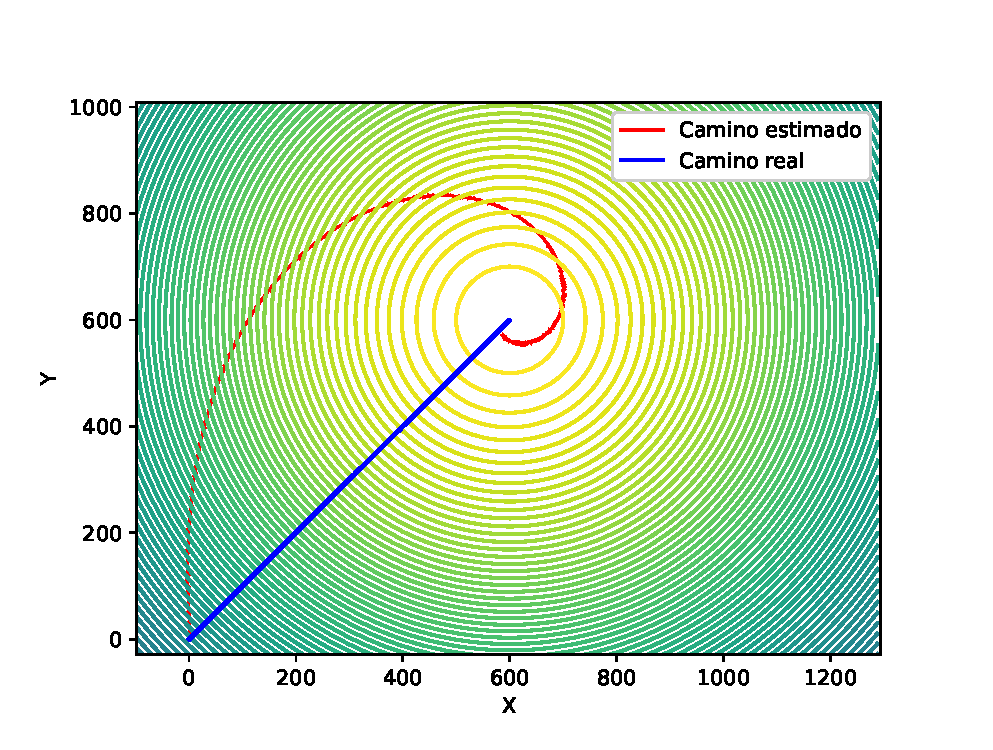
\includegraphics[width=0.75\textwidth]{figures/Caso_Inicial/Caminos.eps}
\caption{Comparativa entre el camino descrito por el gradiente y por el gradiente estimado} \label{Dif_Caminos}
\end{figure}

\begin{figure}[H]
\centering
\includegraphics[width=0.75\textwidth]{figures/Caso_Inicial/Figure_3.eps}
\caption{Comparativa las componentes del gradiente entre el real y el estimado} \label{grad}
\end{figure}

\begin{figure}[H]
\centering
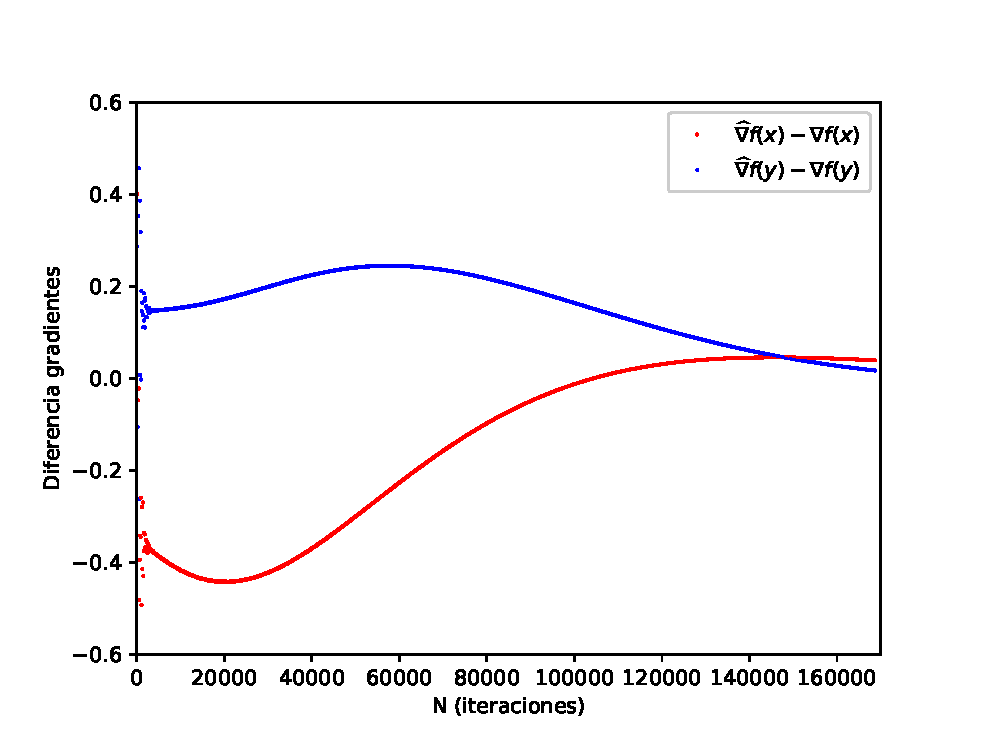
\includegraphics[width=0.75\textwidth]{figures/Caso_Inicial/Figure_4.eps}
\caption{Diferencia entre las componentes del gradiente real y estimada} \label{Dif_grad}
\end{figure}

\begin{figure}[H]
\centering
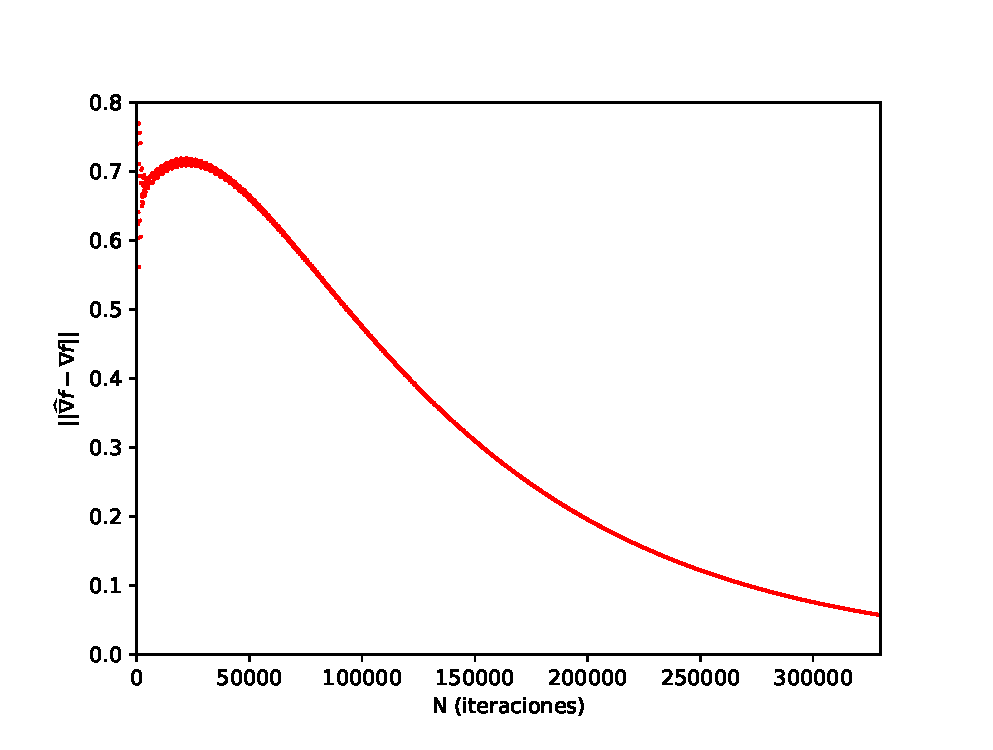
\includegraphics[width=0.75\textwidth]{figures/Caso_Inicial/Figure_5.eps}
\caption{Curva de error descrita por la estimación del gradiente} \label{Curva_error}
\end{figure}
\newpage

Un comentario destacable es que se deben imponer dos condiciones que necesariamente se deben cumplir para que el algoritmo avance satisfactoriamente. Estas son:

\begin{itemize}
	\item La primera es que el error de formación sea lo más próximo a 0 posible, es decir, que en la medida de lo que cabe los vehículos estarán dispuestos simétricamente en el círculo pero con un error que se adicionará al existente por la estima del gradiente. Por ello, se decide imponer que como mucho $e_{\theta}\leq{0.2}$.
	\item La segunda consiste en dar una solución satisfactoria para tomar en consideración que ya se ha llegado al punto de interés. Esto se debe a la dificultad de movimiento cuando estés muy cerca del máximo al aproximarse prácticamente a una recta siendo su derivaba una constante. Por ello, se impone que para satisfacer condición de máximo, es decir, es solución al problema cuando $f(x)\geq{0.999}$.
\end{itemize}

En la figura \ref{Dif_Caminos} se aprecia como claramente el avance obtenido por el gradiente estimado difiere claramente del real pasando de una recta a definir prácticamente una espiral. Esto era un resultado bastante esperable al acumular un error equiparable al orden 2 de Taylor visto en la ecuación \ref{Fun_Esti}, además se le suma el efecto del ascenso de gradiente el cual va a tener un error por cada paso que se da y por ende te iras acercando al máximo con dicha forma. Por otro lado, en la figura \ref{grad} se observa la variación de cada componente para cada una de las iteraciones con respecto al gradiente real frente al estimado, una cosa a tener en cuenta es que al inicio se ve como tanto la componente en x como en y del gradiente real empiezan en $cos(45)$ y $sin(45)$ respectivamente y van variando su valor hasta llegar al punto de máxima concentración de sustancias. Este resultado interesa para poder aproximar al error como la diferencia entre ambos, es decir, lo que se tiene en \ref{Dif_grad}.
\newpage
Recopilando toda esta información y acudiendo a la referencia \cite{Estimacion_Gradiente} el error puede aproximarse como:
\begin{equation} \label{error_gradiente}
	\Delta{\nabla{f\left(c\right)}}=||\hat{\nabla}f\left(c\right)-\nabla{f}\left(c\right)||
\end{equation}

En todas las figuras descritas a lo largo de este capítulo en el eje se dispone de $\nabla{f}$ dado que se presupone que siempre va a estar en el centro, tal como se comento en \ref{Estima}.

La figura \ref{Curva_error} describe el error dado por \ref{error_gradiente}. En este se ve como claramente según se va acercado el conjunto de robots al máximo el error se va disminuyendo y esto se debe a que el valor del gradiente tiende a 0 traduciéndose eso en la ecuación \ref{GA} que el avance es menor. Dicha situación se puede aprovechar para evaluar bajo que condiciones el algoritmo funciona mejor, es decir, tal como se describió al principio del capítulo se tiene que estudiar la relación existente entre $\Delta{\nabla{f\left(c\right)}}$ y $\hat{\nabla}{f\left(c\right)}$ con los diferentes parámetros del sistema.

\section{Variación del punto inicial}

\begin{figure}[H]
\centering
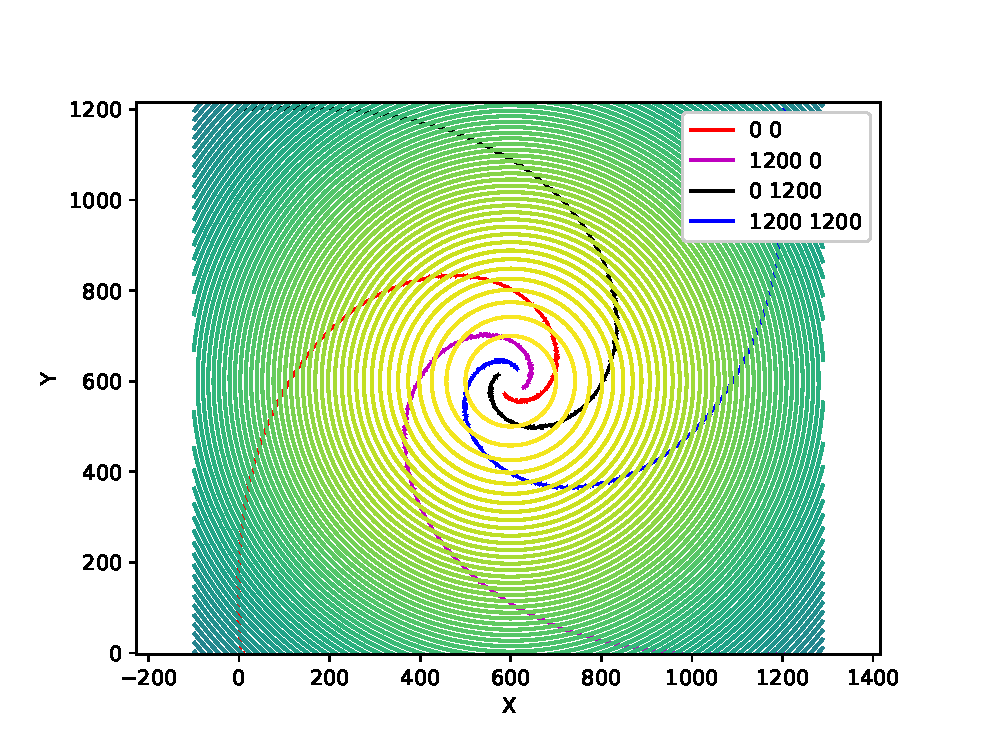
\includegraphics[width=0.70\textwidth]{figures/4_puntos_observar_forma/Figure_1.eps}
\caption{Avance del sistema en diferentes posiciones de la gaussiana} \label{Avance_Posicion}
\end{figure}

Una de las primeras situaciones planteadas es hacer uso de los mismos datos utilizados anteriormente para evaluar el efecto que tiene partir desde diferentes puntos, es decir, en lugar de empezar desde el origen elegir otro punto inicial. Consecuentemente, se escogen los otros 3 vertices que pueden conformar una diagonal con respecto al punto máximo siendo estos $x_o=[0,1200]$, $x_o=[1200,0]$ y $x_o=[1200,1200]$. El resultado esperable es que la trayectoria descrita mantenga la forma, pero evidentemente lo hará pasando por otros puntos definidos en el función. Finalmente, se contempla en la figura \ref{Gradiente_Diversos_Puntos} que las iteraciones se mantienen iguales para cada punto de partida, por ende la forma esperada del error terminaría siendo similar a \ref{Curva_error} en todos los casos. 

\begin{figure}[H]
  \begin{center}
    \subfigure[Punto 0 0]{
        \includegraphics[width=0.45\textwidth]{figures/4_puntos_observar_forma/0_0/Figure_3_INICIO.eps}
        }
    \subfigure[Punto 0 1200]{
        \includegraphics[width=0.45\textwidth]{figures/4_puntos_observar_forma/0_1200/Figure_3_Esquina.eps}
        }
	\subfigure[Punto 1200 0]{
        \includegraphics[width=0.45\textwidth]{figures/4_puntos_observar_forma/1200_0/Figure_3.eps}
        }
	\subfigure[Punto 1200 1200]{
        \includegraphics[width=0.45\textwidth]{figures/4_puntos_observar_forma/1200_1200/Figure_3_1.eps}
        }
    \caption{Evaluación del gradiente estimado en diversos puntos de la gaussiana}
    \label{Gradiente_Diversos_Puntos}
  \end{center}
\end{figure}

\section{Variación del número de agentes N}

\begin{figure}[H]
\centering
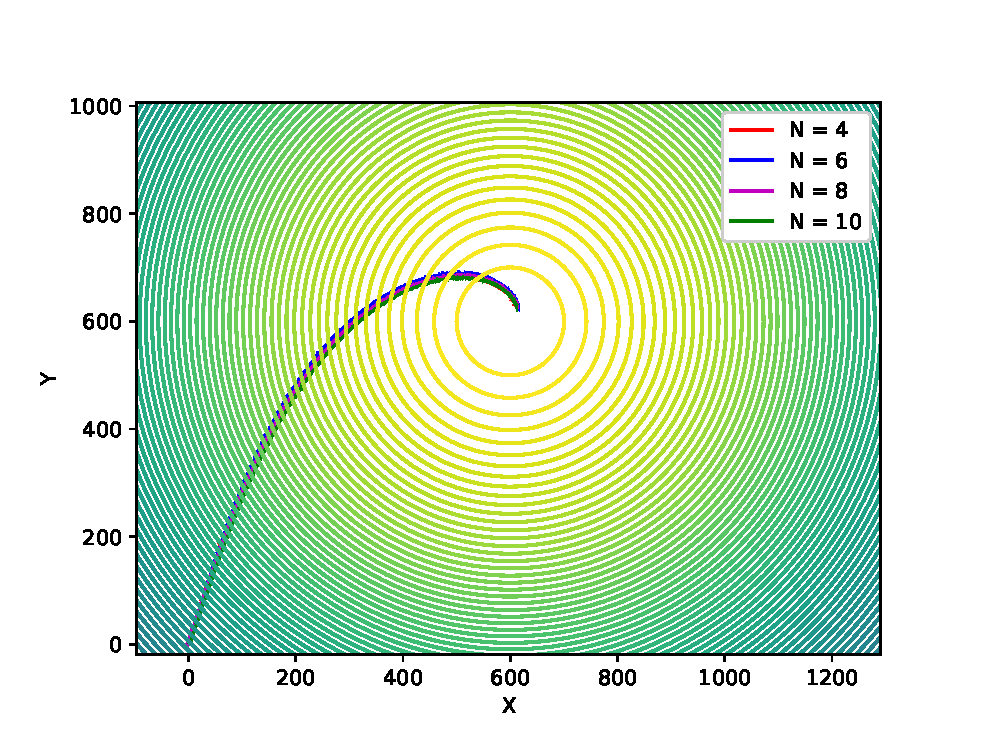
\includegraphics[width=0.70\textwidth]{figures/N_Var_R_50/Figure_1.eps}
\caption{Avance del sistema en función del número de agentes N} \label{N_Var}
\end{figure}

El número de agentes va a influir de dos maneras: 

\begin{enumerate}
	\item Este primer caso directamente sale de leer la ecuación \ref{Fun_Esti} y de la gráfica \ref{NAGENTSEST}, en donde claramente se aprecia una dependencia inversamente proporcional, es decir, a medida que se aumenta el número de agentes es de esperarse que el error se reduzca y a su vez las iteraciones necesarias para llegar al máximos se reducen.
	\item No obstante, si se tiene en cuenta el algoritmo de control de formación esto implicaría que cada vez tu número de agentes va creciendo teniendo más nodos dentro del sistema y por ello se ha de pasar mucha más información al presentar mas nodos adyacentes. A esto se le añade el tiempo que se tendría que esperar para que los N vehículos se dispongan de manera simétrica en la formación.
\end{enumerate}

Para obtener estos resultados se impuso que $D = 50$ y $\epsilon\hspace{2mm}{=20}$. Se puede apreciar como la trayectoria descrita en \ref{N_Var} no cambia significativamente. Sin embargo, si tiene un impacto en el número de iteraciones \ref{Gradiente_N_Var} y en la reducción del error \ref{N_Var_Error}. Para este último caso, se tiene que a partir de un determinado número de agentes el sistema se vuelve invariante, es decir, existe un valor de N límite para la reducción del error.

\begin{figure}[H]
  \begin{center}
    \subfigure[N = 4]{
        \includegraphics[width=0.45\textwidth]{figures/N_Var_R_50/N=4/Figure_3.eps}
        }
    \subfigure[N = 6]{
        \includegraphics[width=0.45\textwidth]{figures/N_Var_R_50/N=6/Figure_3.eps}
        }
	\subfigure[N = 8]{
        \includegraphics[width=0.45\textwidth]{figures/N_Var_R_50/N=8/Figure_3.eps}
        }
	\subfigure[N = 10]{
        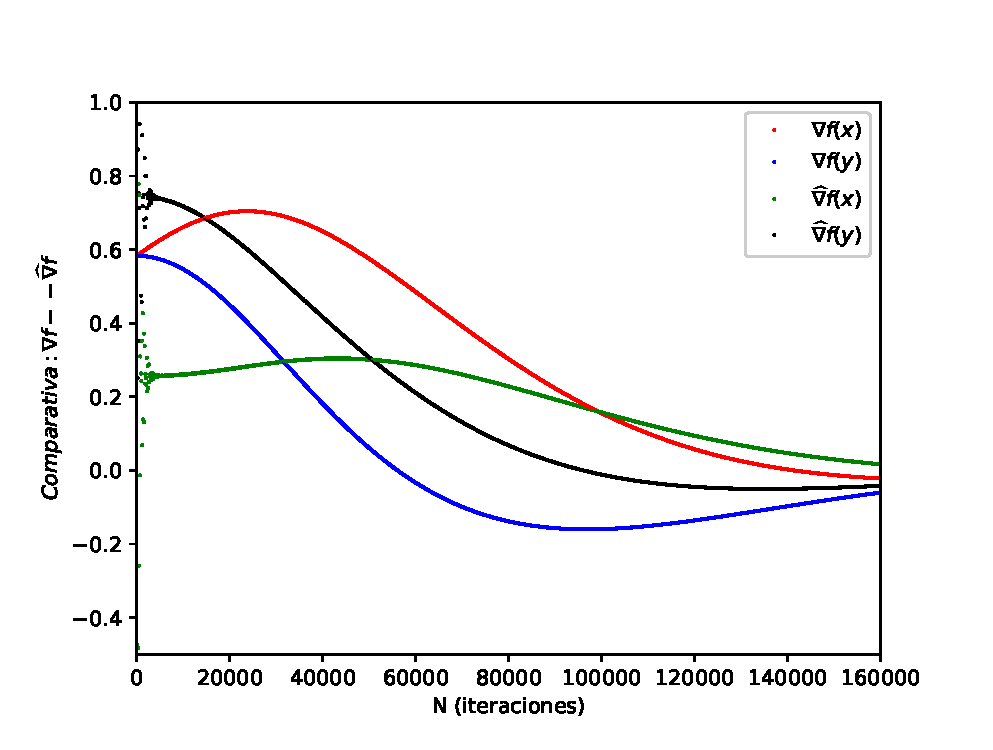
\includegraphics[width=0.45\textwidth]{figures/N_Var_R_50/N=10/Figure_3.eps}
        }
    \caption{Evaluación del gradiente estimado en función del número de agentes N}
    \label{Gradiente_N_Var}
  \end{center}
\end{figure}

Adicionalmente, se aprecia que el valor de ambas componentes del gradiente va a oscilar cuando el valor de la función no es próximo a 1 y el número de agentes es relativamente pequeño.

\begin{figure}[H]
\centering
\includegraphics[width=0.70\textwidth]{figures/N_Var_R_50/Figure_5.eps}
\caption{Error descrito por el gradiente al variar el número de agentes N} \label{N_Var_Error}
\end{figure}

\section{Variación del radio D}

\begin{figure}[H]
\centering
\includegraphics[width=0.70\textwidth]{figures/Dif_R_BU/Figure_1.eps}
\caption{Avance del sistema en función del radio D} \label{D_Var}
\end{figure}

Imponiendo que N = 4 y $\epsilon$=20, se evalúa la influencia del radio D:

\begin{enumerate}
	\item Retomando \ref{Fun_Esti} se observa que la función es inversamente proporcional al cuadrado de D. Esto implica que al aumentar el radio provoca que el gradiente estimado disminuya significativamente conllevando a que la trayectoria descrita por este se parezca cada vez más a la trazada por el gradiente real. Esto se aprecia en la figura \ref{Gradiente_Var_D}.
	\item En la formación de control va a influir directamente el radio de la circunferencia dado que entre mayor sea D el error prefijado será menos restrictivo y por ende aprecias comportamientos oscilantes en las zonas lejanas al máximo de radiación.
\end{enumerate}

\begin{figure}[H]
  \begin{center}
    \subfigure[D = 30]{
        \includegraphics[width=0.45\textwidth]{figures/Inicio_0_0/N4_R30_E20/Figure_3.eps}
        }
    \subfigure[D = 40]{
        \includegraphics[width=0.45\textwidth]{figures/Dif_R_BU/N4_R40_E20_BU/Figure_3.eps}
        }
	\subfigure[D = 50]{
        \includegraphics[width=0.45\textwidth]{figures/Dif_R_BU/N4_R50_E20_BU/Figure_3.eps}
        }
	\subfigure[D = 60]{
        \includegraphics[width=0.45\textwidth]{figures/Dif_R_BU/N4_R60_E20_BU/Figure_3.eps}
        }
    \caption{Evaluación del gradiente estimado y el real en función del radio D}
    \label{Gradiente_Var_D}
  \end{center}
\end{figure}

Comparando directamente \ref{N_Var_Error} y \ref{D_Var_Error}, se observa una mayor influencia del valor de D sobre el de N. Evaluando únicamente al radio D se ve como a medida que su valor decrece el error aumenta y con ello el número de iteraciones de una forma mucho mas notoria que el número de agentes. 

\begin{figure}[H]
\centering
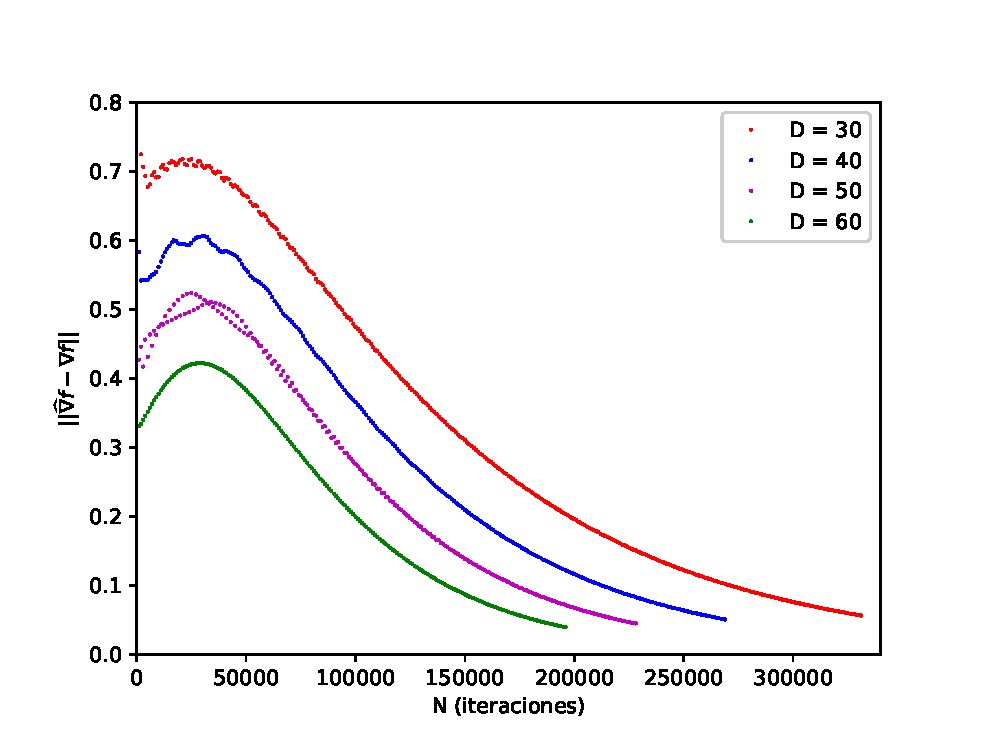
\includegraphics[width=0.70\textwidth]{figures/D_Var/D_variable.eps}
\caption{Error descrito por el gradiente al variar el radio D} \label{D_Var_Error}
\end{figure}

\section{Variación del peso $\epsilon$}

Este caso va a estar estrictamente relacionado con \ref{GA} dado que si se aumenta el valor de $\epsilon$ es de esperarse que el gradiente tome un valor más alto y uno se platea que posiblemente llegue más rápido al punto máximo. No obstante, al aumentar el peso que multiplica al gradiente a su vez estas arrastrando al error provocando que la espiral se acentué mucho más. Este efecto es apreciable en la \ref{Epsilon_Var}

\begin{figure}[H]
\centering
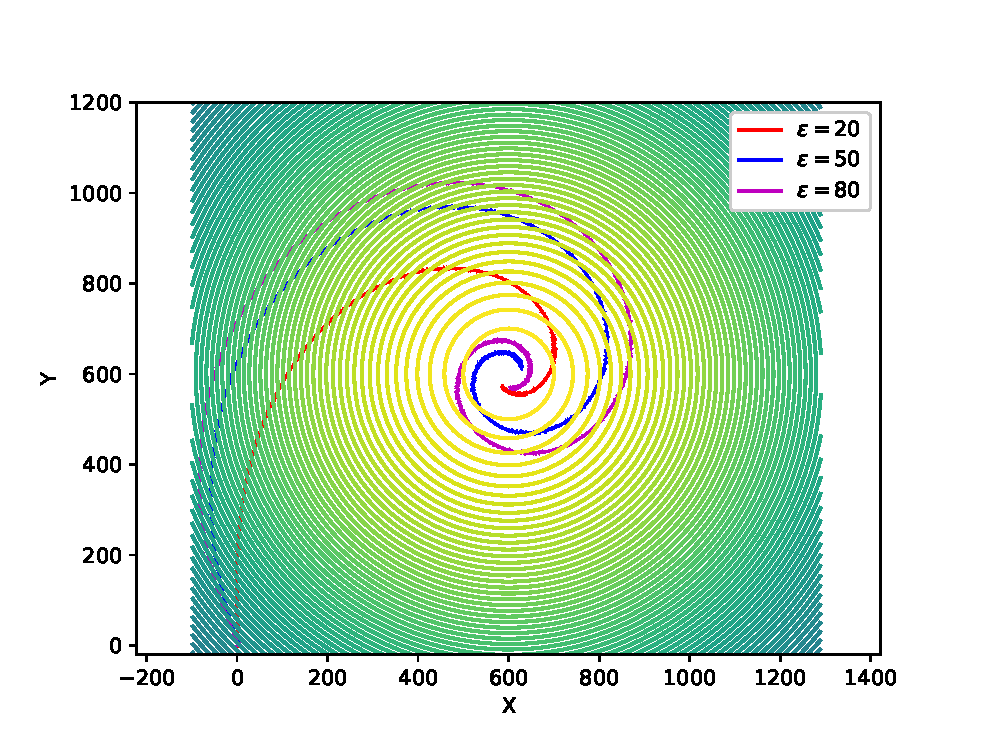
\includegraphics[width=0.72\textwidth]{figures/Epsilon_variante/Figure_1.eps}
\caption{Avance del sistema en función del radio peso $\epsilon$} \label{Epsilon_Var}
\end{figure}

\begin{figure}[H]
\centering
\includegraphics[width=0.72\textwidth]{figures/Epsilon_variante/Figure_5.eps}
\caption{Error descrito por el gradiente al variar el peso $\epsilon$} \label{Epsilon_Var_Error}
\end{figure}

Se observa en la figura \ref{Epsilon_Var_Error} que aumentar el peso $\epsilon$ es perjudicial para el algoritmo dado que un aumento significativo de este valor conllevaría a elevar en exceso tanto el número de iteraciones como $\Delta{\nabla{f\left(c\right)}}$. Este efecto era justo el contrario cuando se tenia el gradiente real, es decir, si aumentabas el valor de dicho peso se daban casos donde llegabas con menos pasos al máximo. Se destaca que para obtener estas simulaciones se hizo uso de $N = 4$ y $D = 30$

\begin{figure}[H]
  \begin{center}
    \subfigure[$\epsilon$ = 20]{
        \includegraphics[width=0.41\textwidth]{figures/Epsilon_variante/e=20/Figure_3.eps}
        }
    \subfigure[$\epsilon$ = 50]{
        \includegraphics[width=0.41\textwidth]{figures/Epsilon_variante/e=50/Figure_3.eps}
        }
	\subfigure[$\epsilon$ = 80]{
        \includegraphics[width=0.41\textwidth]{figures/Epsilon_variante/e=80/Figure_3.eps}
        }
    \caption{Evaluación del gradiente en función del peso $\epsilon$}
    \label{Gradiente_Var_Epsilon}
  \end{center}
\end{figure}

Finalmente, se procederá a evaluar un caso particular en el que se tienen múltiples fuentes emitiendo con el objetivo de demostrar las limitaciones que presenta la utilización del algoritmo de ascenso de gradiente.

\section{Evaluación con Múltiples fuentes}

En este caso se va a considerar que N = 4, D = 50 y $\epsilon$=20, además el nuevo plano sobre el que se desplaza el enjambre se describe según:

\begin{itemize}
	\item Una función gaussiana que va presentar el máximo valor de sustancia con $p=1$, va a estar rotada $45º$ es por ello que la simetría sobre el plano se tiene que retocar haciendo que sobre el eje x se tenga mucha mas desviación que sobre el eje y, esto se logra mediante la multiplicación por matrices de rotación al producto matricial anteriormente descrito $H=X^{T}\cdot{S}\cdot{X}$ con una desviación de $\bigl[\begin{smallmatrix}S_{xx} & S_{xy}\\ S_{yx} & S_{yy}\end{smallmatrix}\bigr]$ donde $S_{xx}=\frac{1000}{\sqrt{2}}$, $S_{yy}=\frac{500}{\sqrt{2}}$ y $S_{xy}=S_{xy}\neq{0}$ cuyo centro va a estar ubicado en el mismo sitio que en el caso anterior.
	\item Otras dos gaussiana que se encuentran definidas con un valor de $p=0.9$, sin rotación con $S_{xx}=S_{yy}={\frac{300}{\sqrt{2}}}$ y $S_{xy}=S_{yx}={0}$, en donde cada presenta su centro en dos sitios diferentes siendo $c_{2}=[0,1200]$ y $c_{3}=[1200,0]$.
\end{itemize}

Al sumarlas se obtiene:

\begin{figure}[H]
  \begin{center}
    \subfigure[Vista en 3D]{
        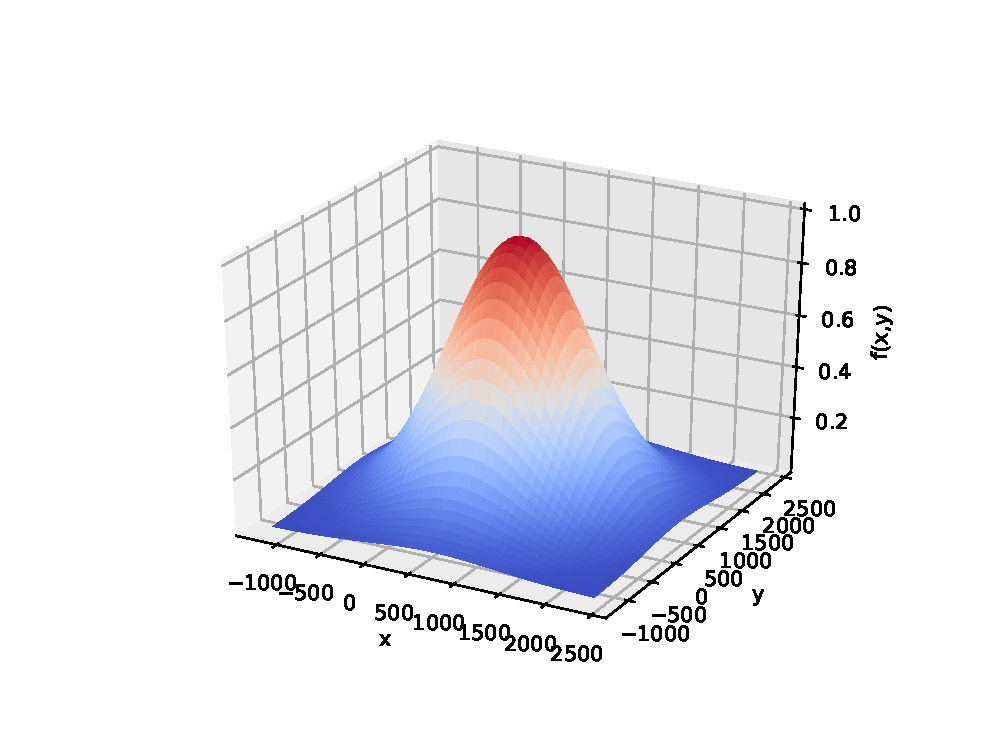
\includegraphics[width=0.45\textwidth]{figures/Casos_Especiales/Gaussiana.eps}
        }
    \subfigure[Curvas de nivel]{
        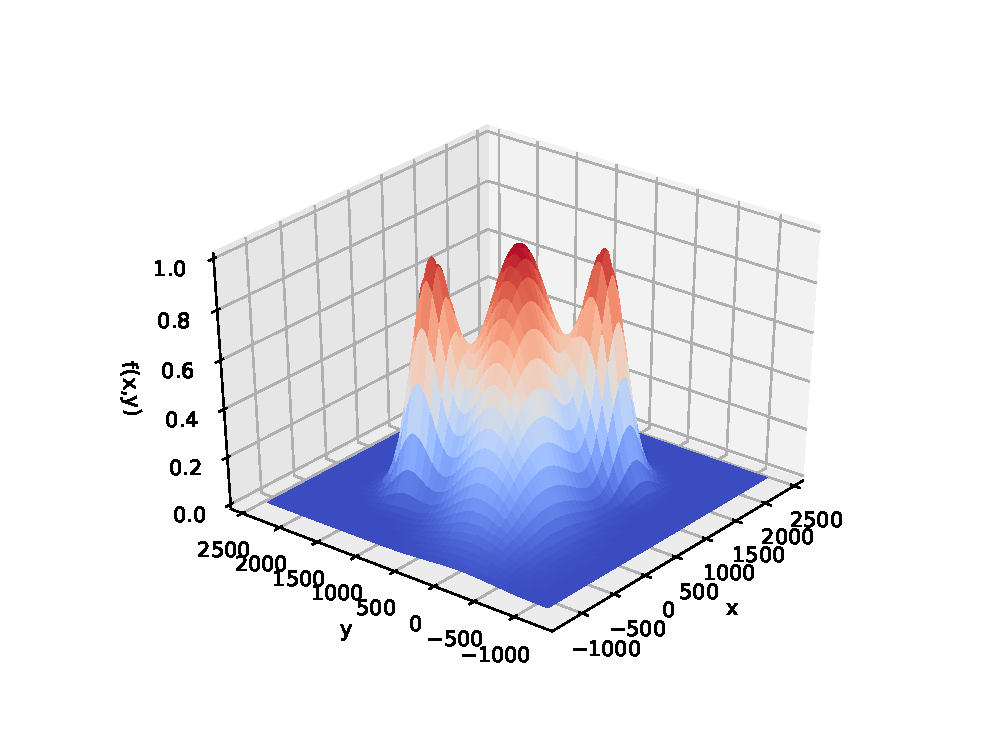
\includegraphics[width=0.45\textwidth]{figures/Casos_Especiales/Gaussiana_meh.eps}
        }
    \caption{Nueva función cuadrática resultado de la suma de 3 gaussianas}
    \label{New_Gaussiana}
  \end{center}
\end{figure}
\newpage
Con esta nueva función surgen dos casos de interés:

\begin{enumerate}
	\item El primero es que se tienen múltiples máximos, en concreto, dos locales y el global. Por lo que puede suceder que dependiendo del número de agentes N, el radio D o el peso $\epsilon$ vaya hacia cualquiera de los tres. Sin embargo, como ya se hizo un estudio para cada uno de ellos directamente se evalúan las posiciones de partida del enjambre para observar hacia que fuente de emisión se dirige.
	\item El segundo son los puntos silla generados entre los tres máximos. Estos haciendo uso del gradiente real conformaban un problema al utilizar el algoritmo de ascenso de gradiente al hacerse $\nabla{f\left(c\right)}=0$. No obstante, se verá que en este caso eso no va a suceder.
\end{enumerate}
	
\begin{figure}[H]
\centering
\includegraphics[width=0.75\textwidth]{figures/Multi_Gaussiana/Figure_1.eps}
\caption{Avance definido sobre el plano con múltiples fuentes en tres puntos diferentes} \label{Multiples_Fuentes}
\end{figure}

\begin{figure}[H]
  \begin{center}
    \subfigure[$f\left(x\right)=0.97$]{
        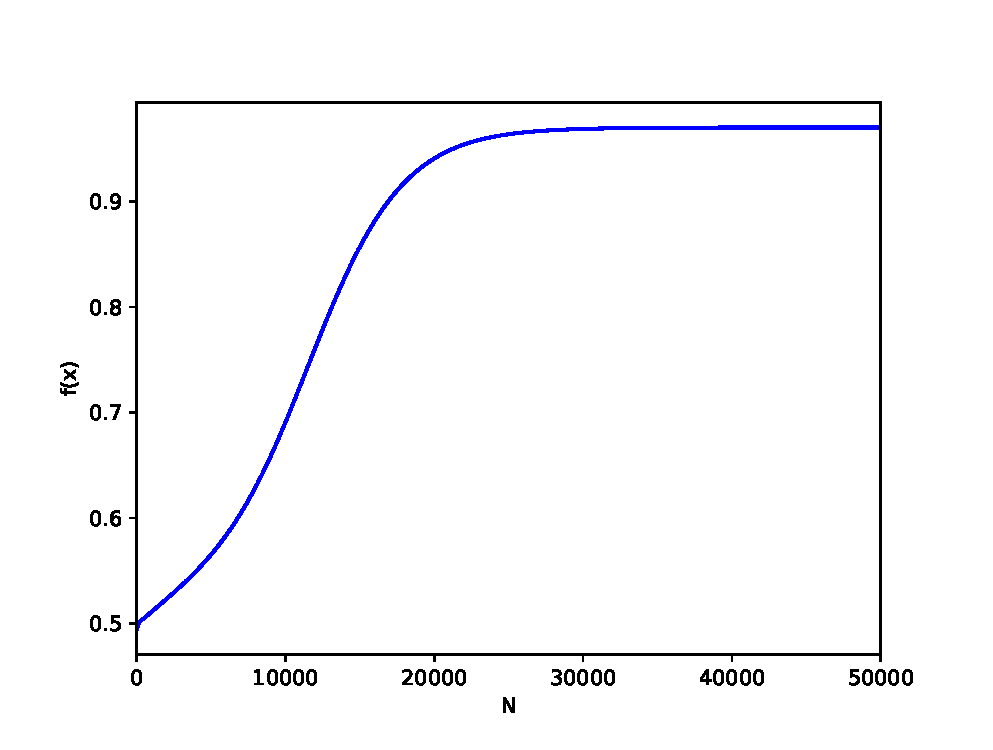
\includegraphics[width=0.45\textwidth]{figures/Multi_Gaussiana/Multi_0_800/Figure_2.eps}
        }
    \subfigure[$f\left(x\right)=1$]{
        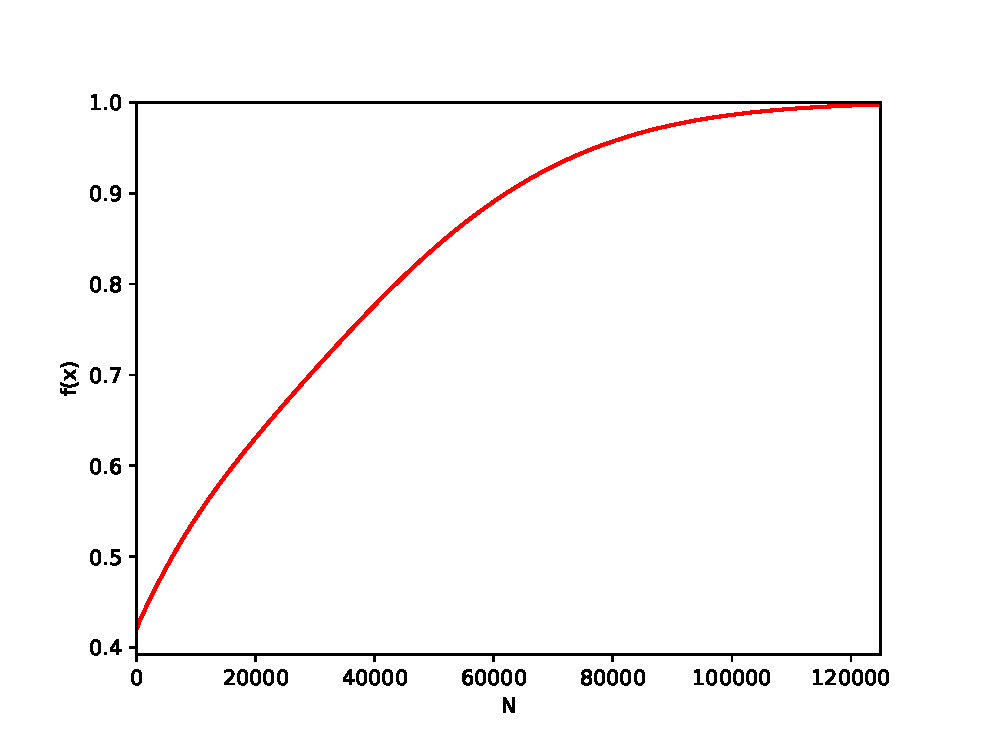
\includegraphics[width=0.45\textwidth]{figures/Multi_Gaussiana/Figure_2.eps}
        }
    \caption{Comparación del valor máximo de ambas fuentes}
    \label{Fun_Gauss_Multi}
  \end{center}
\end{figure}

Comparando los valores obtenidos para los caminos azul y rojo de \ref{Multiples_Fuentes} a partir de la figura \ref{Fun_Gauss_Multi}, se observa como dados dos posiciones iniciales el algoritmo no es capaz de distinguir cual de los dos es el que posee mayor concentración de sustancias. Esto se debe a una limitación del propio algoritmo el cual únicamente te va a estar continuamente elevando el valor de la función hasta encontrar un máximo más no tendrá la capacidad de distinguirlos.

\begin{figure}[H]
  \begin{center}
    \subfigure[Inicio en 0 0]{
        \includegraphics[width=0.45\textwidth]{figures/Multi_Gaussiana/Multi_En_0/Figure_3.eps}
        }
    \subfigure[Inicio en 0 800]{
        \includegraphics[width=0.45\textwidth]{figures/Multi_Gaussiana/Multi_0_800/Figure_3.eps}
        }
    \caption{Evaluación del gradiente estimado y el real según la fuente objetivo}
    \label{Comp_Multi_Gaussian}
  \end{center}
\end{figure}

Una segunda cosa que surge de recorrer los máximos locales es que  definidos de forma plana en el centro, en donde casi definen una recta que anteriormente se dijo que el valor de su derivada era una constante y por ende el avance por dicha zona va a ser prácticamente imposible. Esto se refleja si se observan las componentes del gradiente estimado en la figura \ref{Comp_Multi_Gaussian} estas conforman una recta horizontal que no esta exactamente en cero pero tiende hacia dicho valor, es decir, esta acotada.

Por otro lado, la trayectoria de color rosa en \ref{Multiples_Fuentes} consistía en definir una situación inicial que se encuentre justo sobre el punto silla. En el caso de utilizar el gradiente estimado esto no va a suponer un problema al tener el gradiente un error, en este caso dicho error va a representar una ventaja dado que permite al algoritmo salirse de ese tipo de situaciones, es decir, los puntos sillas pasan desapercibidos gracias a la operación conjunta de los tres algoritmos.





